\documentclass{article}
\usepackage{amsmath}
\usepackage{tikz}
\usepackage{graphicx}
\usepackage{color}
\usepackage{alltt}
\usepackage{tcolorbox}
\usepackage{soul}
\usepackage{xcolor}

\graphicspath{{graphics/}}

\newcommand{\ctext}[3][RGB]{%
      \begingroup
        \definecolor{hlcolor}{#1}{#2}\sethlcolor{hlcolor}%
          \hl{#3}%
            \endgroup
        }

\begin{document}
\title{An Introduction to Geoprocessing with ArcPy}
\maketitle

\section{An Informal Introduction to Geoprocessing}
Most likely, a majority of the GIS work you do in your life (and certainly in this class) will not be cartographic, that is, creating map products.  Instead, it will be work processing geographic data, working with \textit{spatial data} to create \textit{spatial information}.  But this is essentially jargon on the level of ``synergy'' talks that I assume must go on corporate offices around the world.  What's important is that you will be spending a lot of time in the magical (and often frustrating world of ``geoprocessing''.  
\subsection{But What Does Geoprocessing Mean for Me?}
A good working definition for geoprocessing in the context of ArcGis is anything you do with one of the ``tools''.  ``Hey!'', you may be thinking to yourself, ``I've already geoprocessed all sorts of junk!  I've hillshaded and projected and\dots'', you're right that's geoprocessing, but don't close this document yet!  As you do more and more GIS, you'll begin to do geoprocessing that's more complex, involving more files, steps and options.  While you can (usually) get by searching for a tool in ArcMap, running it on one of your files, searching for the next tool, locating the output of the first tool, and running the second tool on that output, etc., there is a much more elegant and powerful way and elegant way to go about it.
\section{Scripting}
\subsection{Making Lists}
Imagine you had an unprojected elevation raster for Oberlin with the NAD83  datum that you wanted to project to UTM with the NAD83 datum, and then make into a hillshade.  If you weren't currently in the GIS lab, you could write out a list of instructions to follow later:
\begin{enumerate}
    \item Project raster
    \item Make hillshade
\end{enumerate}
Unfortunately, you are delayed 6 months and forget which raster you wanted to work with.  This could've been solved with a more detailed list of instructions:
\begin{enumerate}
    \item Project Oberlin elevation raster
    \item Make hillshade
\end{enumerate}
Problem solved?  Alas, this time you were delayed a year and have forgotten where you stored all of your many elevation rasters on your hard drive.  Luckily, this can be solved with an even more detailed list:
\begin{enumerate}
    \item project \verb+F:/gis/elevation_rasters/oberlin_dem.tif+
    \item Make hillshade
\end{enumerate}
However, this time you are delayed 25 years and have forgotten how all these tools work!  So a more detailed list is in order:
\begin{enumerate}
    \item Use the Project Raster tool with the following options: 
          \begin{description}
              \item [Input Raster:] \verb+F:/gis/elevation_rasters/oberlin_dem.tif+
              \item [Output Raster:] \verb+F:/gis/elevation_rasters/oberlin_dem_utm.tif+
              \item [Output Coordinate System:] \verb+NAD_1983_UTM_Zone_17N+
          \end{description}
      \item Use the Hillshade tool with the following options:
            \begin{description}
                \item [Input Raster:] \verb+F:/gis/elevation_rasters/oberlin_dem_utm.tif+
                \item [Output Raster:] \verb+F:/gis/hillshades/oberlin.tif+
            \end{description}
\end{enumerate}
What a list!  Sure, it's detailed, but now you could give this list and your hard drive to anyone with a little ArcGIS experience and they could do it for you.  However, I must admit it seems unlikely that you will be delayed for 25 years on your way to the GIS lab (and if you are, you have bigger problems than making a hillshade!), and making a list with this level of detail to give to someone else might not save a whole lot of your time.  

\subsection{Lists for Computers}
Scripting is essentially writing lists of instructions, like the ones above, that a computer will follow, preforming each instruction one by one.  This involves learning how to write lists that computers can understand, but becomes a real time saver and a powerful tool.  With scripts (list of instructions written for computers) multi-step processes can be automated and reused.  Scripts can be incredibly simple and incredible complex, but even the simplest ones can be massive time savers.

\section{Scripting for ArcGIS}
When writing scripts (instruction lists) for ArcGIS you will write in the style used by the Python programming language.  This doesn't mean you will need to learn how to \textit{program} with Python, simply how to write instruction lists in a way that Python understands.  There are three main things you need to know about writing lists that Python can understand, first: that Python executes each step in order; second, how to tell Python to run tools, and third, how to name pieces of information so that you can refer to them later.  We will illustrate these three things by looking at a pre-written script.
\subsection{Calculating Sinuosity With a Script}
\subsubsection{Sinuosity}
You will be using a script to calculate the sinuosity of the river features you digitized earlier in the lab.  Sinuosity is defined as follows: 
\begin{equation*}
    \frac{\text{the length of the path of the river}}{\text{the distance between each end of the river}}
\end{equation*}
or graphically:
\begin{equation*}
    \frac{
          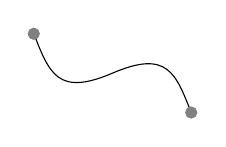
\begin{tikzpicture}
              \draw (0,1) .. controls (.2, .5) and (.3, .2) .. (1, .5)
                          .. controls (1.7, .8) and (1.8, .5) .. (2, 0);
              \filldraw[gray] (0,1) circle [radius=2pt]
                              (2,0) circle [radius=2pt];
          \end{tikzpicture}
      }{
          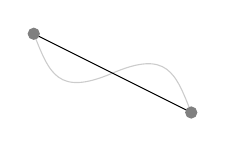
\begin{tikzpicture}
             \draw[black!20] (0,1) .. controls (.2, .5) and (.3, .2) .. (1, .5)
                               .. controls (1.7, .8) and (1.8, .5) .. (2,0);
              \draw (0,1) -- (2,0);
              \filldraw[gray] (0,1) circle [radius=2pt]
                              (2,0) circle [radius=2pt];
          \end{tikzpicture}
       }
\end{equation*}
Since the length of river's path can never be shorter than the distance between the ends, the minimum sinuosity value will be 1.

\subsubsection{The sinuosity script}
\begin{enumerate}
    \item First, you need to get the sinuosity script.
        \begin{enumerate}
            \item Use the internet to search for a script to calculate sinuosity in ArcGIS.  You should find a result on ArcGIS.com which has something for you to download.
            \item Download and extract the zip file.  
            \item Find the file called \verb+Sinousity.pyt+.  A \verb+.pyt+ file is a special type of Python file that ArcGIS can use like a toolbox.  
        \end{enumerate}
    \item Now, run the script
        \begin{enumerate}
            \item Go into the ArcCatalog window and navigate to the \verb+pyt+ file.  Expand the toolbox and open the Calculate Sinuosity tool.  
            \item Run the tool on your digitized river path shapefile.  
        \end{enumerate}
    \item It should have added a new field in the attribute table with the sinuosity of the river.  However, the value is less than one!  It turns out, the sinuosity tool is calculating inverse sinuosity.  While it would be easy to simply fix the result, lets use this as learning opportunity and fix the script instead.  
        \begin{enumerate}
            \item Open the program IDLE (Python GUI).
            \item In IDLE, open up the Sinuosity toolbox.

                You will have to change ``Files of Type'' to ``All files''.
                \\\includegraphics[width=\linewidth]{allfiles}
                Be sure that the type of the file you are opening is ``Python Toolbox''
                \\\includegraphics[width=\linewidth]{type}
        \end{enumerate}
\end{enumerate}
\vspace{2mm}
Wow.  There is a lot going on here.  However, only a few lines are the script itself, the rest is code dedicated into making it a tool that you can run graphically in ArcMap.  The important part is the four lines below \verb+def getSinuosity(shape):+

\noindent
\includegraphics[width=\textwidth]{getsinuosity}
Take special note of the second and third lines:

\noindent
\includegraphics[width=\textwidth]{doubleline}
Notice the indentation.  This is really one line split into two lines simply to increase readability.  So what we have is a list with three steps, the one starting with ``\verb+length+'', the one starting with ``\verb+d+'', and the one starting with ``\verb+return+''.  Lets take them one at a time.
\begin{enumerate}
    \item \verb+length = shape.length+
        This line tells Python to label a piece of information.  Python uses the \verb+=+ character to label things.  This line says ``use `\verb+length+' to refer to `\verb+shape.length+', a label defined elsewhere that refers to length of the shape the tool is running on.  
    \item \verb+d = math.sqrt(...)+
        This line is somewhat more complex.  From \verb+d = ...+ we can see that there is an instruction to label something with ``\verb+d+'', however \textit{what} is being labeled seems rather obtuse.  For now lets focus on the sets of parentheses.  
        \begin{alltt}
d = math.sqrt\colorbox{cyan}{(\colorbox{yellow}{(shape.firstPoint.X - shape.lastPoint.X)} ** 2 +}
              \colorbox{cyan}{\colorbox{orange}{(shape.firstPoint.Y - shape.lastPoint.Y)} ** 2)}
\end{alltt}
There are three sets of parentheses, the \textcolor{cyan}{cyan} parentheses, which encompasses both the \textcolor{yellow}{yellow} and \textcolor{orange}{orange} parentheses.  The text in between the cyan parentheses is a math expression, with labels like \verb+shape.firstPoint.X+ filling in for numbers.  The yellow and orange parentheses are there to ensure correct order of operations in the math expression.  
So far, we can understand this instruction as ``use `\verb+d+' to refer to \\*`\verb+math.sqrt([math expression])+' ''

But just what is up with \verb+math.sqrt(...)+ anyway?  \verb+math.sqrt+ is a tool, like hillshade or project raster.  The parentheses specify what should be used as input to the tool.  In this case, the tool calculates the square root, and its input is math expression.  So this instruction can be read as ``run the square root tool on the given math expression and give the result the label `\verb+d+'.''
    \item \verb+return d / length+
        This instruction has two components, \verb+return+ and \verb+d / length+.  \verb+d / length+ is a simple math expression, divide the number that the label \verb+d+ represents by the number that the label \verb+length+ represents.  You don't need to worry about the \verb+return+ component, it simply means take the result of the division operation and make it available for use elsewhere in the script.
\end{enumerate}
Now that you've looked at each instruction, you should be able to figure out what to change to make the script calculate sinuosity as we've defined it.  Make the change, save the file, and re-navigate to and run the tool.
Congratulations!  You've just worked with your first ArcPy script, and are well on your way to making your own.
\end{document}
